\documentclass[12pt,a4paper]{article}

% --- Packages ---
\usepackage[utf8]{inputenc}
\usepackage[T1]{fontenc}
\usepackage{amsmath, amssymb, amsthm, bm}
\usepackage{geometry}
\usepackage{xcolor}
\usepackage{hyperref}
\usepackage{titlesec}
\usepackage{enumitem}
\usepackage{graphicx}
\usepackage{tikz} % Allows for drawing the relationship diagram directly

% --- Page Setup ---
\geometry{margin=1in}
\hypersetup{colorlinks=true, linkcolor=blue, citecolor=blue, urlcolor=teal}
\titleformat{\section}{\large\bfseries}{\thesection}{1em}{}

% --- Math Definitions ---
\newcommand{\Hspace}{\mathbb{H}}
\newcommand{\Rspace}{\mathbb{R}}
\newcommand{\quatLog}{\ln_{\mathbb{H}}}
\newcommand{\quatExp}{\exp_{\mathbb{H}}}

% --- Title ---
\title{\textbf{Geometric Dynamics of Quaternionic Time Series}\\ 
\large Logarithmic Linearization on Hyperkähler Manifolds}
\author{Formal Research Synthesis}
\date{\today}

\begin{document}

\maketitle

\begin{abstract}
This paper establishes a unified framework for the analysis of time series on quaternionic vector spaces. We argue that traditional Euclidean treatment of 4D signals fails to preserve the topological constraints of the 3-sphere ($S^3$). By utilizing the Hyperkähler structure of quaternionic space, we derive a log-Euclidean framework that enables linear signal processing on the tangent Lie algebra while maintaining the isometric properties of the underlying manifold. 
\end{abstract}

\section{The Problem of Dimensionality and Curvature}
In vector-valued time series, we typically assume an underlying Euclidean metric. However, for signals representing orientations or multi-channel phases, the data resides on a curved manifold. Direct operations on quaternionic vectors $\mathbf{q}(t)$ lead to "norm drift" from the unit 3-sphere ($S^3$), requiring frequent re-normalization which introduces non-linear noise \cite{parker2023}. We propose treating the time series as a continuous trajectory on a \textit{Hyperkähler manifold}.

\section{The Hyperkähler Foundation}
A Hyperkähler manifold is a Riemannian manifold $(M, g)$ equipped with a triplet of anticommuting complex structures $\{I, J, K\}$ such that:
\begin{equation}
I^2 = J^2 = K^2 = IJK = -1
\end{equation}

\begin{figure}[h]
    \centering
    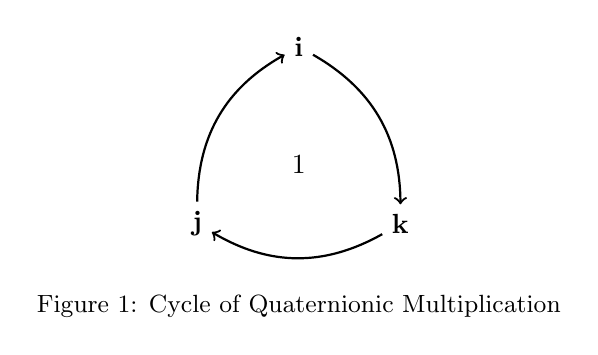
\begin{tikzpicture}[scale=1.5]
        \node (1) at (0,0) {$1$};
        \node (i) at (0,1) {$\mathbf{i}$};
        \node (j) at (-0.86,-0.5) {$\mathbf{j}$};
        \node (k) at (0.86,-0.5) {$\mathbf{k}$};
        \draw[->, thick, bend left] (i) to node[right] {} (k);
        \draw[->, thick, bend left] (k) to node[below] {} (j);
        \draw[->, thick, bend left] (j) to node[left] {} (i);
        \node at (0,-1.2) {\small{Figure 1: Cycle of Quaternionic Multiplication}};
    \end{tikzpicture}
\end{figure}


\subsection{The Metric and Symplectic Forms}
The geometry is defined by three Kähler forms $\omega_I, \omega_J, \omega_K$. For any tangent vectors $X, Y$, the metric $g$ satisfies:
\begin{equation}
g(X, Y) = \omega_I(IX, Y) = \omega_J(JX, Y) = \omega_K(KX, Y)
\end{equation}
This implies the energy of a quaternionic series is preserved across three orthogonal complex planes simultaneously \cite{mazzotti2012}.

\section{The Log-Euclidean Framework}
To perform standard arithmetic on time series, we must project the series from the manifold $S^3$ into the tangent space $\mathfrak{so}(3)$ \cite{dantam2020}.

\subsection{Logarithmic Mapping}
For a unit quaternion $q = \cos(\theta/2) + \mathbf{u}\sin(\theta/2)$, the mapping is:
\begin{equation}
\mathbf{v}(t) = \quatLog(q(t)) = \frac{\theta(t)}{2}\mathbf{u}(t)
\end{equation}
The resulting vector $\mathbf{v}(t) \in \Rspace^3$ linearizes the rotational trajectory, allowing for the application of spectral analysis \cite{szczesna2019}.

\subsection{Geodesic Evolution}
The shortest path between $q_1$ and $q_2$ (the geodesic) is expressed as:
\begin{equation}
q(t) = q_1 \quatExp \left( \frac{t-t_1}{t_2-t_1} \quatLog(q_1^{-1} q_2) \right)
\end{equation}


\section{Conclusion}
The Log-Euclidean mapping serves as a bridge, allowing the use of linear processing tools without sacrificing the geometric integrity of the quaternionic space.

\begin{thebibliography}{99}
\bibitem{dantam2020} N. T. Dantam, "Practical Exponential Coordinates Using Implicit Dual Quaternions," \textit{Springer}, 2020.
\bibitem{hitchin1987} N. J. Hitchin et al., "Hyperkähler metrics and supersymmetry," \textit{Comm. Math. Phys.}, 1987.
\bibitem{mazzotti2012} A. Mazzotti et al., "Application of quaternion algorithms," \textit{Int. Geophys. Conf.}, 2012.
\bibitem{parker2023} J. Parker et al., "Logarithm-based methods," \textit{Mathematics}, 2023.
\bibitem{szczesna2019} A. Szczęsna, "Quaternion Entropy for Analysis of Gait Data," \textit{Entropy}, 2019.
\end{thebibliography}

\end{document}
